
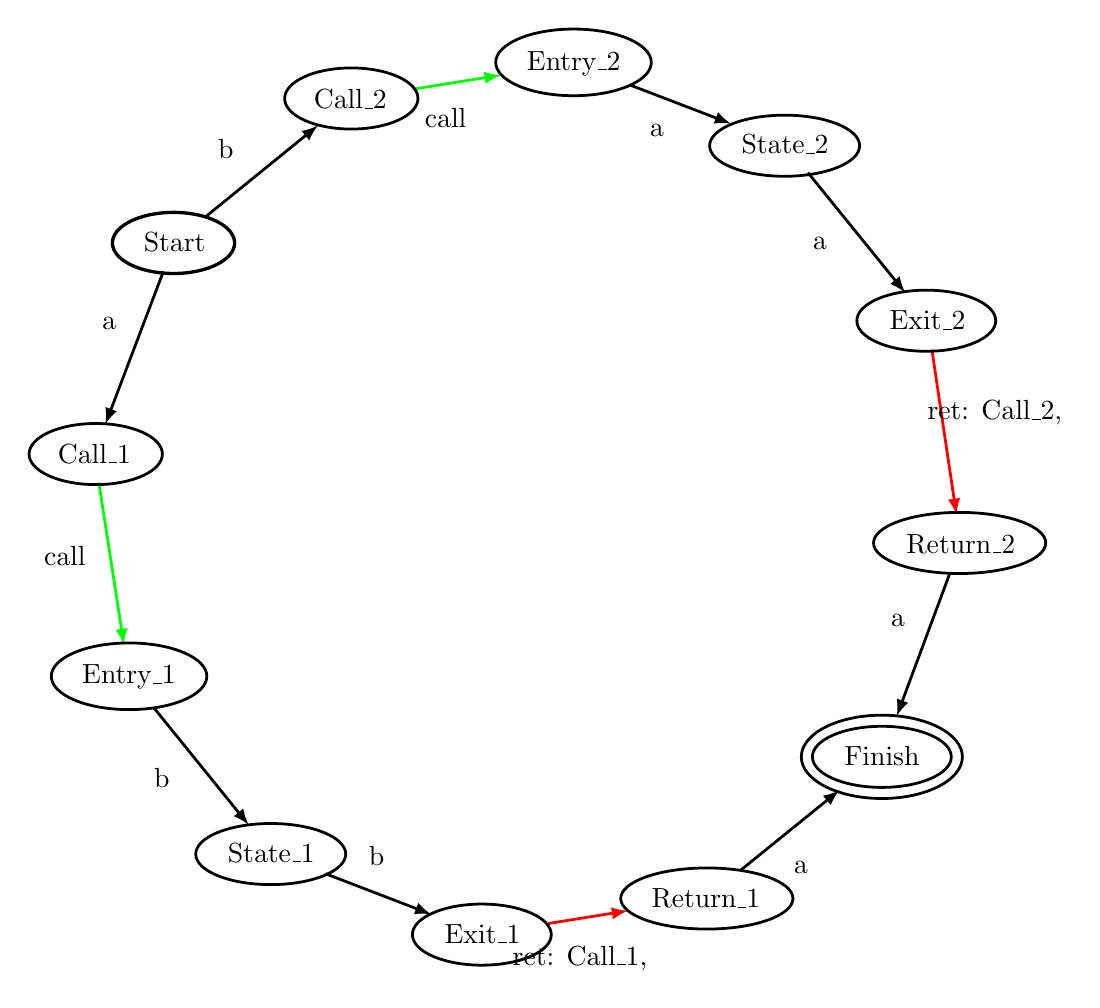
\begin{tikzpicture}[>=latex,line join=bevel,]
  \pgfsetlinewidth{1bp}
%%
\pgfsetcolor{black}
  % Edge: Return_1 -> Finish
  \draw [->] (257.88bp,41.958bp) .. controls (265.78bp,48.351bp) and (276.32bp,56.877bp)  .. (293.71bp,70.955bp);
  \definecolor{strokecol}{rgb}{0.0,0.0,0.0};
  \pgfsetstrokecolor{strokecol}
  \draw (279.83bp,43.244bp) node {a};
  % Edge: Exit_2 -> Return_2
  \pgfsetcolor{red}
  \draw [->] (327.01bp,229.64bp) .. controls (328.87bp,217.1bp) and (332.03bp,195.86bp)  .. (335.85bp,170.16bp);
  \definecolor{strokecol}{rgb}{0.0,0.0,0.0};
  \pgfsetstrokecolor{strokecol}
  \draw (349.69bp,206.85bp) node {ret: Call\_2, };
  % Edge: Call_1 -> Entry_1
  \pgfsetcolor{green}
  \draw [->] (27.127bp,181.72bp) .. controls (29.021bp,169.46bp) and (32.201bp,148.9bp)  .. (36.155bp,123.32bp);
  \definecolor{strokecol}{rgb}{0.0,0.0,0.0};
  \pgfsetstrokecolor{strokecol}
  \draw (14.875bp,155.47bp) node {call};
  % Edge: State_2 -> Exit_2
  \draw [->] (282.38bp,293.32bp) .. controls (290.06bp,283.85bp) and (301.67bp,269.52bp)  .. (317.39bp,250.11bp);
  \draw (286.64bp,267.72bp) node {a};
  % Edge: State_1 -> Exit_1
  \draw [->] (108.78bp,40.902bp) .. controls (117.47bp,37.564bp) and (127.85bp,33.575bp)  .. (146.77bp,26.307bp);
  \draw (127.06bp,47.418bp) node {b};
  % Edge: Return_2 -> Finish
  \draw [->] (333.46bp,149.02bp) .. controls (329.47bp,138.29bp) and (323.15bp,121.31bp)  .. (314.4bp,97.773bp);
  \draw (314.7bp,132.17bp) node {a};
  % Edge: Start -> Call_2
  \draw [->] (65.695bp,277.55bp) .. controls (74.667bp,284.84bp) and (87.422bp,295.19bp)  .. (106bp,310.28bp);
  \draw (72.871bp,301.69bp) node {b};
  % Edge: Call_2 -> Entry_2
  \pgfsetcolor{green}
  \draw [->] (140.47bp,323.39bp) .. controls (147.02bp,324.44bp) and (154.34bp,325.61bp)  .. (171.77bp,328.4bp);
  \definecolor{strokecol}{rgb}{0.0,0.0,0.0};
  \pgfsetstrokecolor{strokecol}
  \draw (151.98bp,313.07bp) node {call};
  % Edge: Start -> Call_1
  \draw [->] (50.37bp,257.79bp) .. controls (45.929bp,246.08bp) and (38.672bp,226.96bp)  .. (29.482bp,202.74bp);
  \draw (30.755bp,239.08bp) node {a};
  % Edge: Entry_1 -> State_1
  \draw [->] (46.871bp,100.72bp) .. controls (54.551bp,91.235bp) and (65.775bp,77.368bp)  .. (81.05bp,58.495bp);
  \draw (49.803bp,75.51bp) node {b};
  % Edge: Entry_2 -> State_2
  \draw [->] (218.85bp,324.66bp) .. controls (226.97bp,321.55bp) and (236.42bp,317.93bp)  .. (254.68bp,310.94bp);
  \draw (228.02bp,308.62bp) node {a};
  % Edge: Exit_1 -> Return_1
  \pgfsetcolor{red}
  \draw [->] (188.93bp,23bp) .. controls (194.83bp,23.943bp) and (201.31bp,24.978bp)  .. (217.6bp,27.583bp);
  \definecolor{strokecol}{rgb}{0.0,0.0,0.0};
  \pgfsetstrokecolor{strokecol}
  \draw (200.32bp,10.5bp) node {ret: Call\_1, };
  % Node: Finish
\begin{scope}
  \definecolor{strokecol}{rgb}{0.0,0.0,0.0};
  \pgfsetstrokecolor{strokecol}
  \draw (309bp,83bp) ellipse (25bp and 11bp);
  \draw (309bp,83bp) ellipse (29bp and 15bp);
  \draw (309.03bp,83.352bp) node {Finish};
\end{scope}
  % Node: Return_2
\begin{scope}
  \definecolor{strokecol}{rgb}{0.0,0.0,0.0};
  \pgfsetstrokecolor{strokecol}
  \draw (337bp,160bp) ellipse (31bp and 11bp);
  \draw (337.41bp,159.63bp) node {Return\_2};
\end{scope}
  % Node: Start
\begin{scope}
  \definecolor{strokecol}{rgb}{0.0,0.0,0.0};
  \pgfsetstrokecolor{strokecol}
  \draw [very thick] (54bp,268bp) ellipse (22bp and 11bp);
  \draw (54.387bp,268.37bp) node {Start};
\end{scope}
  % Node: Return_1
\begin{scope}
  \definecolor{strokecol}{rgb}{0.0,0.0,0.0};
  \pgfsetstrokecolor{strokecol}
  \draw (246bp,32bp) ellipse (31bp and 11bp);
  \draw (245.67bp,32.07bp) node {Return\_1};
\end{scope}
  % Node: Entry_2
\begin{scope}
  \definecolor{strokecol}{rgb}{0.0,0.0,0.0};
  \pgfsetstrokecolor{strokecol}
  \draw (198bp,333bp) ellipse (28bp and 12bp);
  \draw (198.06bp,332.62bp) node {Entry\_2};
\end{scope}
  % Node: Exit_2
\begin{scope}
  \definecolor{strokecol}{rgb}{0.0,0.0,0.0};
  \pgfsetstrokecolor{strokecol}
  \draw (325bp,240bp) ellipse (25bp and 11bp);
  \draw (325.44bp,240.17bp) node {Exit\_2};
\end{scope}
  % Node: Entry_1
\begin{scope}
  \definecolor{strokecol}{rgb}{0.0,0.0,0.0};
  \pgfsetstrokecolor{strokecol}
  \draw (38bp,112bp) ellipse (28bp and 12bp);
  \draw (37.943bp,111.75bp) node {Entry\_1};
\end{scope}
  % Node: State_1
\begin{scope}
  \definecolor{strokecol}{rgb}{0.0,0.0,0.0};
  \pgfsetstrokecolor{strokecol}
  \draw (89bp,48bp) ellipse (27bp and 11bp);
  \draw (89.201bp,48.425bp) node {State\_1};
\end{scope}
  % Node: Call_2
\begin{scope}
  \definecolor{strokecol}{rgb}{0.0,0.0,0.0};
  \pgfsetstrokecolor{strokecol}
  \draw (118bp,320bp) ellipse (24bp and 11bp);
  \draw (117.64bp,319.72bp) node {Call\_2};
\end{scope}
  % Node: Call_1
\begin{scope}
  \definecolor{strokecol}{rgb}{0.0,0.0,0.0};
  \pgfsetstrokecolor{strokecol}
  \draw (26bp,192bp) ellipse (24bp and 11bp);
  \draw (25.5bp,192.24bp) node {Call\_1};
\end{scope}
  % Node: State_2
\begin{scope}
  \definecolor{strokecol}{rgb}{0.0,0.0,0.0};
  \pgfsetstrokecolor{strokecol}
  \draw (274bp,303bp) ellipse (27bp and 11bp);
  \draw (274.14bp,303.49bp) node {State\_2};
\end{scope}
  % Node: Exit_1
\begin{scope}
  \definecolor{strokecol}{rgb}{0.0,0.0,0.0};
  \pgfsetstrokecolor{strokecol}
  \draw (165bp,19bp) ellipse (25bp and 11bp);
  \draw (165.24bp,19.211bp) node {Exit\_1};
\end{scope}
%
\end{tikzpicture}
